\section{实验结果}
可执行代码见源码,使用方法见源码中的README,源码可从github上查看下载,地址https://github.com/zhang-x-z/CompilerPrincipal-Lab


测试选取了解析JSON文件中的Token,包括string,\{,\},number,[,],:,逗号,true,null,false以及空格(包括制表符换行),输入的xml文件如下
\begin{lstlisting}
<?xml version="1.0" encoding="UTF-8"?>
<Lex>
    <userDefinitions></userDefinitions>
    <reDefinitions>
        <digit>
            [0-9]
        </digit>
    </reDefinitions>
    <rules>
        <rule>
            <re>
                "(\\.|[^\\"\n])*"
            </re>
            <action>
                cout &lt;&lt; "STRING" &lt;&lt; endl;
            </action>
        </rule>
        <rule>
            <re>
                \{
            </re>
            <action>
                cout &lt;&lt; "LEFT BRACE" &lt;&lt; endl;
            </action>
        </rule>
        <rule>
            <re>
                }
            </re>
            <action>
                cout &lt;&lt; "RIGHT BRACE" &lt;&lt; endl;
            </action>
        </rule>
        <rule>
            <re>
                ,
            </re>
            <action>
                cout &lt;&lt; "COMMA" &lt;&lt; endl;
            </action>
        </rule>
        <rule>
            <re>
                :
            </re>
            <action>
                cout &lt;&lt; "COLON" &lt;&lt; endl;
            </action>
        </rule>
        <rule>
            <re>
                \[
            </re>
            <action>
                cout &lt;&lt; "LEFT BRACKET" &lt;&lt; endl;
            </action>
        </rule>
        <rule>
            <re>
                ]
            </re>
            <action>
                cout &lt;&lt; "RIGHT BRACKET" &lt;&lt; endl;
            </action>
        </rule>
        <rule>
            <re>
                [\r\t \n]
            </re>
            <action>
                cout &lt;&lt; "WIGHTSPACE" &lt;&lt; endl;
            </action>
        </rule>
        <rule>
            <re>
                [1-9]{digit}*|0
            </re>
            <action>
                cout &lt;&lt; "INT" &lt;&lt; endl;
            </action>
        </rule>
        <rule>
            <re>
                ([1-9]{digit}*\.{digit}*)|(0\.{digit}*)
            </re>
            <action>
                cout &lt;&lt; "FLOAT" &lt;&lt; endl;
            </action>
        </rule>
        <rule>
            <re>
                true
            </re>
            <action>
                cout &lt;&lt; "TRUE" &lt;&lt; endl;
            </action>
        </rule>
        <rule>
            <re>
                false
            </re>
            <action>
                cout &lt;&lt; "FALSE" &lt;&lt; endl;
            </action>
        </rule>
        <rule>
            <re>
                null
            </re>
            <action>
                cout &lt;&lt; "NULL" &lt;&lt; endl;
            </action>
        </rule>
    </rules>
    <userCode></userCode>
</Lex>
\end{lstlisting}
配置文件如下
\begin{lstlisting}
buffer_size=60
source_file_location=./test.xml
encoding=utf8
charset=ascii
\end{lstlisting}
测试用JSON文件:
\lstset{language=json}
\begin{lstlisting}
{
    "name": "ZXZ",
    "age": 21,
    "GPA": 3.92,
    "is_male": true,
    "is_famale": false,
    "courses": [
        "Database", "CompilePrincipal", null
    ]
}
\end{lstlisting}
最后输出结果如图:\\
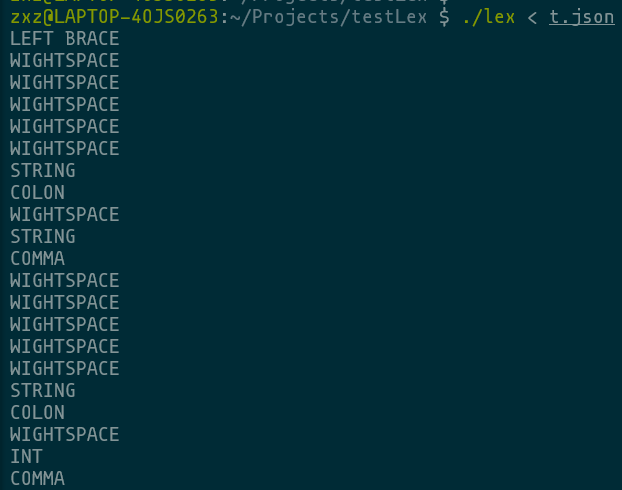
\includegraphics[scale=0.8]{1.png}\\
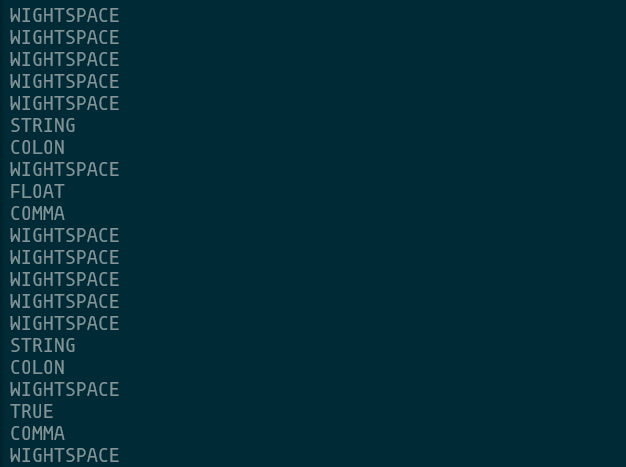
\includegraphics[scale=0.8]{2.png}\\
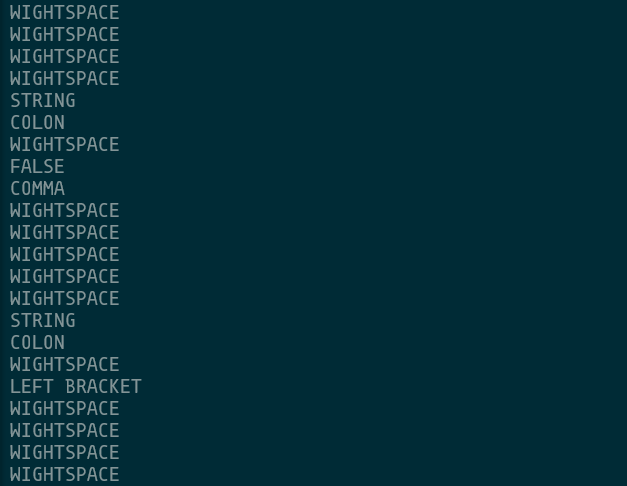
\includegraphics[scale=0.8]{3.png}\\
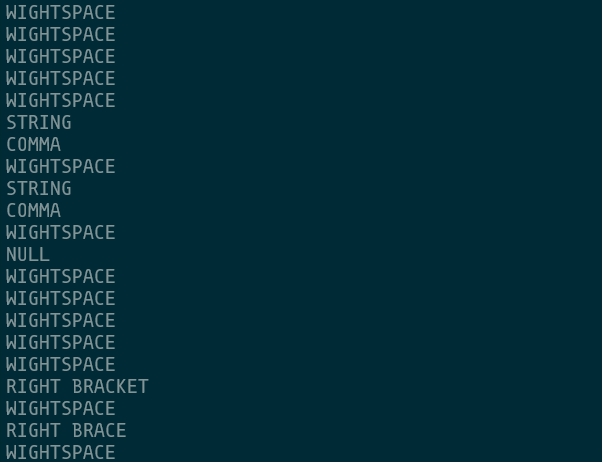
\includegraphics[scale=0.8]{4.png}